\documentclass{article}

\usepackage[francais]{babel}
\usepackage[T1]{fontenc}
\usepackage{moreverb}       % verbatim with tab

\usepackage{wrapfig}
\usepackage{graphicx}
\usepackage{geometry}
\geometry{hmargin=2.5cm}
\usepackage{amsmath}
\usepackage{siunitx}

\usepackage{graphicx}
\usepackage{subcaption}
\usepackage{float}
\usepackage{hyperref}
\usepackage{setspace}
\usepackage{xcolor}
\usepackage{pdfpages}
\usepackage{enumitem}
\usepackage{lscape}

\usepackage{fancyhdr}       % en-têtes
\usepackage{lastpage}       % numéro de dernière page

\title{Réseaux industriels}
\date{2020}
\author{Laura Bin}

\pagestyle{fancy}
\renewcommand\headrulewidth{1pt}
\fancyhead[L]{Laura Binacchi}
\fancyhead[C]{Réseaux industriels}
\fancyhead[R]{\today}

\begin{document}
    \pagenumbering{arabic}

    \begin{center}
        \textbf{\LARGE Travail sur les transferts de fichiers}
    \end{center}

    \paragraph{}
    Réaliser un mini serveur et un mini client de type FTP possédant les caractéristiques suivantes :
    \begin{itemize}
        \item Lorsqu’un client se connectera, le serveur enverra la liste des fichiers downloadables situés dans un dossier précis du serveur (à déterminer au préalable). Les fichiers peuvent être de tous formats et de toutes tailles possibles. Le serveur attendra ensuite du client le nom du fichier à downloader et enverra le fichier au client. Il faudra veiller à optimiser le serveur afin que le transfert soit le plus rapide possible (utiliser une API adéquate pour minimiser les changements de contexte usespace/kernel (cf. cours : \href{https://man7.org/linux/man-pages/man2/sendfile.2.html}{\texttt{sendfile()}}).
        \item Le client recevra l’adresse du serveur sur la ligne de commande. Une fois la connexion réalisée, le client affichera la liste des fichiers du serveur et demandera d’entrer le nom d’un fichier à downloader (ou un numéro correspondant au fichier désiré). Le fichier reçu sera enregistré sur le disque du client.
    \end{itemize}

    \section{Protocole}
    \paragraph{}
    La connexion est engagée par le client en envoyant un byte d'identification au serveur. Ce byte permet de vérifier que le client parle bien le bon protocole. Il pourrait aussi permettre au serveur de sélectionner un autre protocole en envoyant un byte d'identification différent.

    \paragraph{}
    Si le byte d'identification n'est pas celui attendu, le serveur ferme la connexion mais reste à l'écoute de nouvelles connexions. Sinon, il répond avec la liste des fichiers téléchargeables préfixée de sa taille. Ces fichiers sont ceux auxquels le serveur a accès en lecture dans le sous-répertoire \emph{files}.

    \paragraph{}
    Si le dossier \emph{files} ne contient aucun fichier, aucun fichier accessible au serveur ou qu'il n'existe pas, le serveur envoie une liste vide (un préfixe à 0 qui n'est suivi de rien) puis ferme la connexion. Le client affiche un message d'erreur et s'arrête.

    \paragraph{}
    Après réception d'une liste valide, le client attend le choix de fichier de l'utilisateur : le nombre correspondant au fichier lors de l'affichage de la liste. Une nouvelle liste ne contenant que les informations sur ce fichier est envoyée au serveur.

    \paragraph{}
    Le serveur renvoie ce fichier préfixé de sa taille en utilisant \emph{sendfile}.

    \paragraph{}
    Le client reçoit ce fichier et l'écrit par morceaux de taille fixe définie dans les constantes afin de ne pas stocker en mémoire vive la totalité du fichier si celui-ci est trop volumineux. Les fichiers sont téléchargés dans le sous-répertoire \emph{download} relatif à l'endroit à partir duquel le client a été lancé. Si le fichier existe déjà dans le dossier \emph{download}, il est écrasé.

    \section{Compilation}
    \paragraph{}
    Pour la sérialisation des données, j'ai repris la librairie \emph{libserial} précédemment développée. Je l'ai mise à jour à cause d'un bug découvert lors de mes tests et j'utilise maintenant la version 1.1. Pour la mise en place des connexions TCP, j'ai repris la librairie \emph{libtcp} dont j'ai amélioré les codes d'erreurs : ce projet utilise donc la version 2.0 de la librairie.

    \paragraph{}
    Comme pour les projets précédents, j'ai compilé mon code en local en exécutant \texttt{gmake ex-files} à la racine de mes projets. J'ai ensuite copié le client et le serveur sur les machines virtuelles et je les ai rendus exécutables avec \texttt{chmod +x}. J'ai enfin ajouté les versions mises à jour de mes librairies au dossier \emph{lib} et j'ai recréé les liens symboliques avec \texttt{ldconfig -n .}.

    \paragraph{}
    J'obtient les structures de fichiers suivantes sur mes machines virtuelles :
    \begin{verbatimtab}
        - ex-files
            client     | server
            + download | + files
        + ex-lib
        + ex-serial
        - lib
            libserial.so.1 -> libserial.so.1.1
            libserial.so.1.1
            libtcp.so.1 -> libtcp.so.1.0
            libtcp.so.1.0
            libtcp.so.2 -> libtcp.so.2.0
            libtcp.so.2.0
    \end{verbatimtab}

    \section{Tests}
    \subsection{Cas nominal}
    \paragraph{}
    Je teste le téléchargement d'un fichier simple sans avoir préalablement créé le dossier \emph{download} :
    \begin{figure}[H]
        \centering
        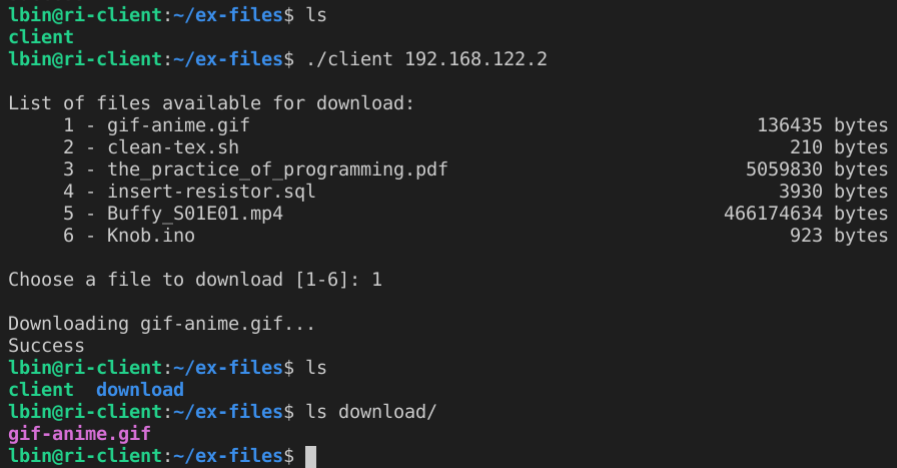
\includegraphics[width=.7\textwidth]{./screenshots/cas-nominal-client.png}
    \end{figure}
    \paragraph{}
    Le dossier a bien été créé et le fichier téléchargé s'y trouve.

    \paragraph{}
    Côté serveur, tout s'est bien déroulé :
    \begin{figure}[H]
        \centering
        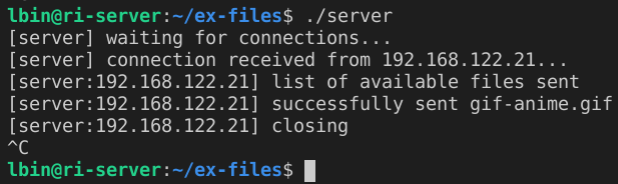
\includegraphics[width=.5\textwidth]{./screenshots/cas-nominal-server.png}
    \end{figure}

    \paragraph{}
    Pour vérifier que les deux fichiers sont identiques, je télécharge le fichier d'origine sur le client avec \texttt{scp} et j'exécute un \texttt{diff}. Le code de retour du diff est 0. Les deux fichiers sont bien identiques.
    \begin{figure}[H]
        \centering
        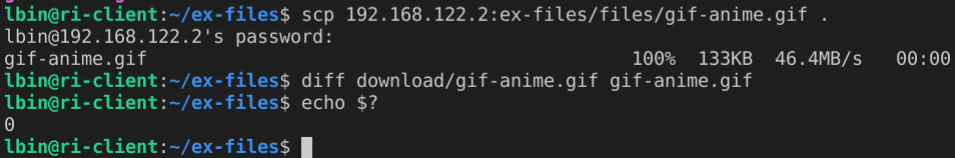
\includegraphics[width=.8\textwidth]{./screenshots/cas-nominal.png}
    \end{figure}


    \subsection{Envoi d'un gros fichier}
    \paragraph{}
    Parmi les différents fichiers testés, j'ai testé le téléchargement d'un fichier de 3.1 GB :

    \begin{figure}[H]
        \centering
        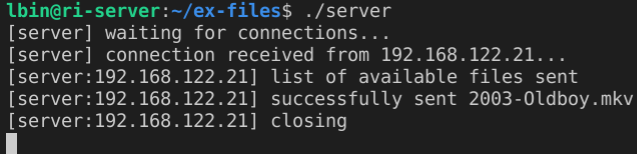
\includegraphics[width=.5\textwidth]{./screenshots/test-big-file-server.png}
    \end{figure}

    \begin{figure}[H]
        \centering
        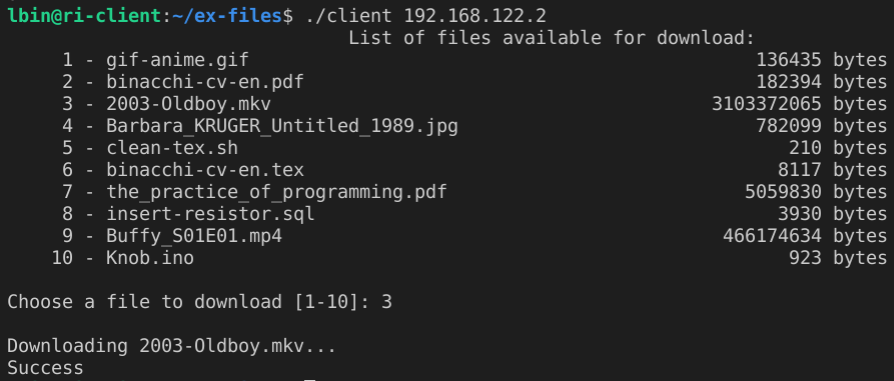
\includegraphics[width=.7\textwidth]{./screenshots/test-big-file-client.png}
    \end{figure}

    \newpage
    \paragraph{}
    Le code de retour du diff est 0. Les deux fichiers sont bien identiques.
    \begin{figure}[H]
        \centering
        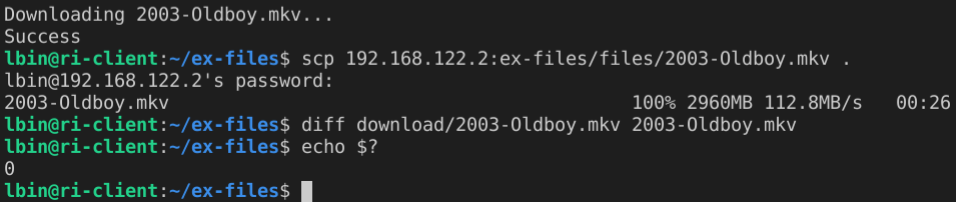
\includegraphics[width=.8\textwidth]{./screenshots/test-big-file.png}
    \end{figure}

    \subsection{Envoi d'un mauvais byte d'identification}
    \paragraph{}
    Si un mauvais byte d'identification est envoyé au serveur, ce dernier ferme la connexion mais reste à l'écoute de nouvelles connexions :
    \begin{figure}[H]
        \centering
        \begin{subfigure}[b]{.48\textwidth}
            \centering
            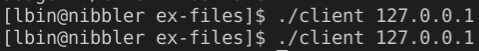
\includegraphics[width=.8\textwidth]{./screenshots/test-wrong-id-client.png}
        \end{subfigure}
        \begin{subfigure}[b]{.48\textwidth}
            \centering
            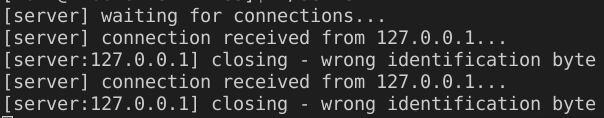
\includegraphics[width=\textwidth]{./screenshots/test-wrong-id-server.png}
        \end{subfigure}
    \end{figure}

    \subsection{Aucun fichier téléchargeable}
    \paragraph{}
    Si le dossier contenant les fichiers téléchargeables n'existe pas sur le serveur, il envoie une liste vide au client puis ferme la connexion mais reste à l'écoute de nouvelles connexions. Le client affiche un message d'erreur avant de s'arrêter. Ce test donne les mêmes résultats si le dossier existe mais ne contient aucun fichier ou si il ne contient aucun fichier accessible en lecture pour le serveur.
    \begin{figure}[H]
        \centering
        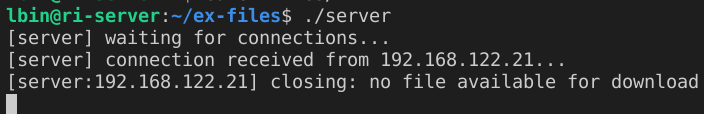
\includegraphics[width=.6\textwidth]{./screenshots/test-no-dir-server.png}
    \end{figure}
    \begin{figure}[H]
        \centering
        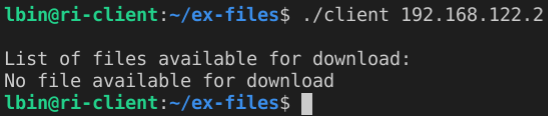
\includegraphics[width=.45\textwidth]{./screenshots/test-no-dir-client.png}
    \end{figure}

    \paragraph{}
    Puisque le serveur reste à l'écoute de nouvelles connexions, il est possible d'ajouter le dossier \emph{files} avec des fichiers pour qu'une nouvelle connection d'un client fonctionne :
    \begin{figure}[H]
        \centering
        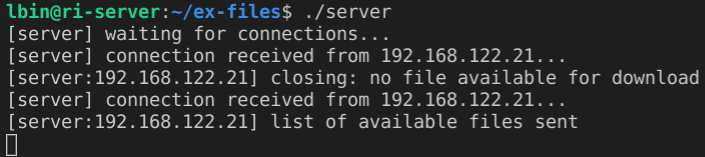
\includegraphics[width=.6\textwidth]{./screenshots/test-add-dir-server.png}
    \end{figure}
    \begin{figure}[H]
        \centering
        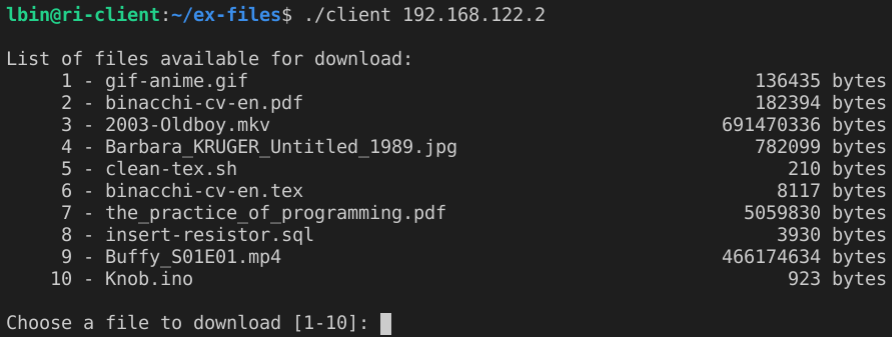
\includegraphics[width=.8\textwidth]{./screenshots/test-add-dir-client.png}
    \end{figure}

    \subsection{Inputs invalides}
    \paragraph{}
    Lorsque l'utilisateur choisi un fichier à télécharger, seul un nombre entier entre 1 et la taille de la liste est accepté, sinon un message d'erreur est affiché. Si l'utilisateur appuie juste sur \texttt{enter}, rien ne se passe. Si un nombre entier est suivi d'autres nombres entiers ou de caractères, seul le premier nombre entier est pris en compte.
    \begin{figure}[H]
        \centering
        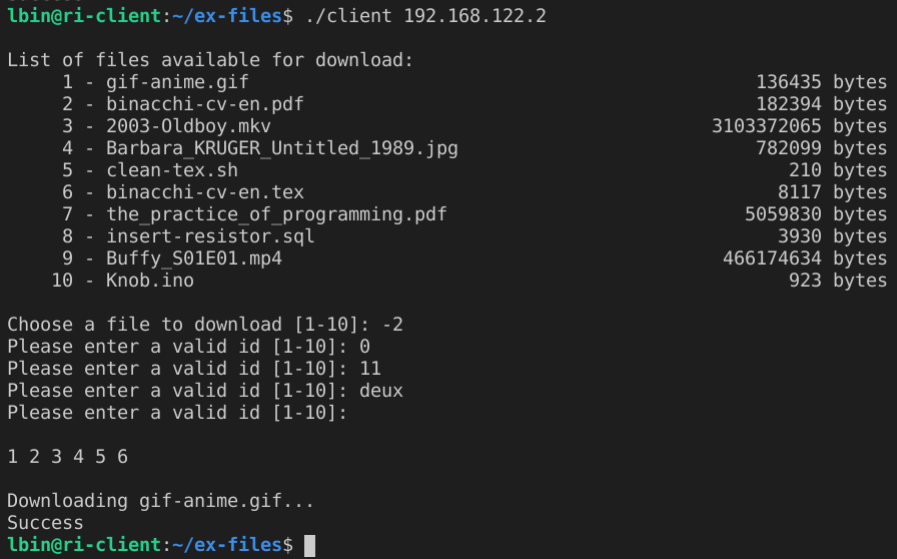
\includegraphics[width=.8\textwidth]{./screenshots/test-invalid-inputs.png}
    \end{figure}

    \newpage
    \subsection{Tests avec valgrind}
    \paragraph{}
    Enfin j'ai testé mon programme avec valgrind pour vérifier l'abscence de fuites mémoire.

    \paragraph{}
    Ce test m'a permis de mettre en évidence un bug dans la librairie \emph{libserial} : lors de la désérialisation des chaînes de caractère, un \texttt{0} aurait dû être ajouté en fin de chaîne.
    \begin{figure}[H]
        \centering
        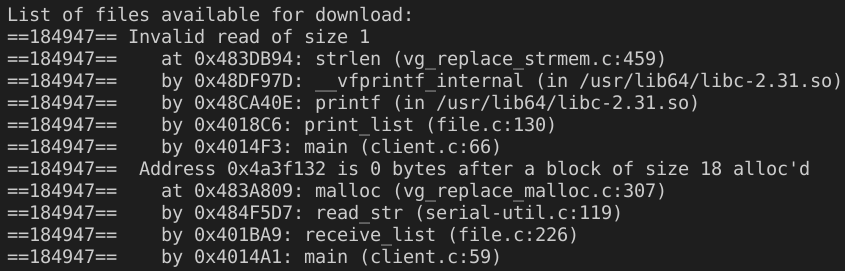
\includegraphics[width=.7\textwidth]{./screenshots/test-valgrind.png}
    \end{figure}

    \paragraph{}
    J'ai donc mis à jour la librairie et sa version.

    \paragraph{}
    Le client libère bien chaque espace de mémoire alloué :
    \begin{figure}[H]
        \centering
        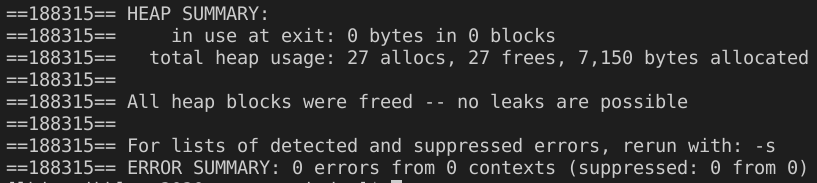
\includegraphics[width=.7\textwidth]{./screenshots/test-valgrind-client.png}
    \end{figure}

    \paragraph{}
    Tout comme le serveur :
    \begin{figure}[H]
        \centering
        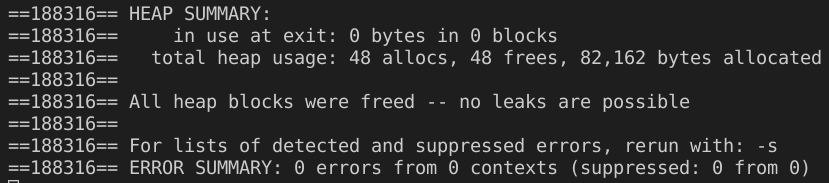
\includegraphics[width=.7\textwidth]{./screenshots/test-valgrind-server.png}
    \end{figure}

\end{document}
\paragraph{}
